\documentclass[11pt,twoside,a4paper]{article}

\usepackage{hyperref}
\usepackage{graphicx}

\begin{document}
  
  \graphicspath{{img//}}
  
  \title{Computer Security \\Revision Notes \\ Ver 0.1 (__GIT_HASH__)}
  \author{Guy Taylor}
  \date{April 2011}
  
  \maketitle
  
  \tableofcontents
  
  \section{Introduction}
    This document is a set of revision notes for the Computer Security \cite{cs_home} course at the Univerisy of Edinbugh.
  
  \clearpage
  
  \begin{section}{Terminology}
    Main buzz words
    \begin{description}
      \item[Cryptography] The secret writing with \emph{ciphers}
      \item[Cryptanalysis] Breaking ciphers
      \item[Cryptology] Both the above
      \item[Encryption] Converting \emph{plain text} to \emph{cipher text}
      \item[Decryption] Converting \emph{cipher text} to \emph{plain text}
      \item[Encryption Scheme, Cipher, Cryptosystem] Mechansisums for encryption and decription
    \end{description}
    
    What is security for
    \begin{description}
      \item[Confidentiality] No agent other than the thows with permision can view the content
      \item[Integrity] The data recived is in fact the data sent
      \item[Authentication] I am who I say I am
      \item[Non-Repudiation] Layered security. Agents with insefisient rights cannot do sertaint things.
    \end{description}
    
    
    Primitives
    \begin{description}
      \item[Plain Text] The unencripted message
      \item[Plain Text] The encripted message
      \item[Key] The secret that needs to be know to encrypt or decrypt a message
      \item[Hash] A \emph{one-way} function. Used so help prevent realeasing the real key.
    \end{description}
    
  \end{section}
  
  \clearpage
  
  \begin{section}{Malises Progams}
    Malware is common
      
      \begin{subsection}{Trojan \emph{Horse}}
        A program that acts beinie such as a game or utility which actualy runs malisshus code while in use as the macerading program.
      \end{subsection}
      
      \begin{subsection}{Virus}
        A program that hides within a normaly unexecutable file (eg pictures, word documents....) that when opened (including previewd by a file manager) causes the parent applicatyion to run malichious code.
      \end{subsection}
      
      \begin{subsection}{Worm}
        A self-replication aplication. The application will try to copy itself over a network or on phisical media (ie USB drives and CDs)
      \end{subsection}
      
      \begin{subsection}{Rootkit}
        A program that embeds itself within the Operating System. This allows it to intersept File System calls to hide itself and apply other coutermesures. These programs are hard to remove as they operate at a lower or simmilar level to Ant-virus scanners.
      \end{subsection}
      
      \begin{subsection}{Loggers}
        Keyloggers and Screenloggers record all screen or keyboard movements. They can include filters so sensative information such as X many keys before and after a credit card (x meany numeric digits). This information is then sent back to a location to be prossesed and missued.
      \end{subsection}
      
      \begin{subsection}{Web Trojan}
        bob
      \end{subsection}
      
      Note: The random term "Crimeware" was used in the lecture notes with only a subsection of the above. All can be used to good or evil so all are "crimeware" if they are used for crime ...
  
  \end{section}
  
  \clearpage
  
  \begin{section}{Phishing and Spoofing}
    TODO
  \end{section}
  
  \clearpage
  
  \begin{section}{Random}
    \begin{figure}[Vom_Noumann_screenshot]
      \centering
      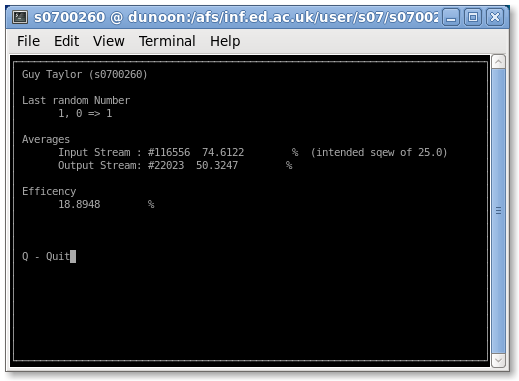
\includegraphics[width=5cm]{von_noumann_screenshot}
      \caption{Screenshot of a skewed random stream been normalised}
    \end{figure}
  \end{section}
  
  \clearpage
  
  \begin{thebibliography}{9}
    \bibitem{cs_home}
      "Computer Security" "\url{http://www.inf.ed.ac.uk/teaching/courses/cs/}"
  \end{thebibliography}

\end{document}
